\chapter{Specifikacija programske potpore}

\section{Funkcionalni zahtjevi}			

\noindent \textbf{Dionici:}

\begin{packed_enum}
	
	\item Ovlašteni zaposlenik tvrtke
	\item Klijent
	\item Administrator
	\item Razvojni tim
	
\end{packed_enum}

\noindent \textbf{Aktori i njihovi funkcionalni zahtjevi:}


\begin{packed_enum}
	\item  \underbar{Neregistrirani/neprijavljeni korisnik (inicijator) može:}
	
	\begin{packed_enum}
		
		\item vidjeti kartu s parkiralištima (adresa, broj ukupnih i slobodnih mjesta, cijena)
		\item registrirati se i/ili prijaviti se (kao klijent ili tvrtka)
		
	\end{packed_enum}
	
	\item  \underbar{Klijent (inicijator) može:}
	
	\begin{packed_enum}
		
		\item vidjeti kartu s parkiralištima (adresa, broj ukupnih i slobodnih mjesta, cijena)
		\item pregledavati, uređivati i izbrisati korisnički račun
		\item pregledavati, uređivati i izbrisati vozila
		\item pregledavati, uređivati i izbrisati karticu
		\item rezervirati parkirališno mjesto
		\item pregledavati, uređivati i izbrisati rezervacije
		\item pisati i pregledavati  recenzije
		\item tražiti upute do parkirališta
		
	\end{packed_enum}
	
	
	\item  \underbar{Ovlašteni zaposlenik tvrtke (inicijator) može:}
	
	\begin{packed_enum}
		
		\item vidjeti kartu s parkiralištima
		\item pregledavati, uređivati, dodavati i brisati svoja parkirališta
		\item pregledavati, uređivati i izbrisati korisnički račun
		\item pregledavati vlastite recenzije
		\item pregledavati rezervacije na vlastitim parkiralištima
		\item odgovoriti na recenzije korisnika
		
	\end{packed_enum}
	
	\item \underbar{Administrator (inicijator) može:}
	
	\begin{packed_enum}
		
		\item vidjeti popis svih registriranih korisnika i osnovnih podataka
		\item pregledavati rezervacije
		\item brisati i mijenjati razinu pristupa aplikaciji drugim korisnicima
		\item brisati recenzije
		\item dodavati ili brisati parkirališta
		
	\end{packed_enum}
	
	\item \underbar{Baza podataka (sudionik) može:}
	
	\begin{packed_enum}
		
		\item pohranjivati podatke o korisnicima (osobni podaci, kartica, vozila)
		\item pohranjivati podatke o parkiralištima (njihovim kapacitetima i ponudama)
		\item pohranjivati podatke o rezervacijama
		\item pohranjivati podatke o tvrtkama
		
	\end{packed_enum}
\end{packed_enum}


\eject 



\subsection{Obrasci uporabe}

\subsubsection{Opis obrazaca uporabe}


\newcounter{uccounter}
\newcommand\showuccounter{\stepcounter{uccounter}\theuccounter}


\noindent \underbar{\textbf{UC\showuccounter\ - Pregled karte}}
\begin{packed_item}
	
	\item \textbf{Glavni sudionik: } Korisnik/Klijent/Tvrtka
	\item \textbf{Cilj:} Pogledati kartu s označenim parkiralištima
	\item \textbf{Sudionici:} Baza podataka
	\item \textbf{Preduvjet:} Korisnik/Klijent/Tvrtka je u aplikaciji
	\item \textbf{Opis osnovnog tijeka:}
	
	\item[] \begin{packed_enum}
		
		\item Korisnik/Klijent/Tvrtka otvara početnu stranicu
		\item Prikazuje se karta s označenim parkiralištima

	\end{packed_enum}
	
\end{packed_item}

\noindent \underbar{\textbf{UC\showuccounter\ - Pregled podataka o parkiralištu na karti}}
\begin{packed_item}
	
	\item \textbf{Glavni sudionik:} Korisnik/Klijent/Tvrtka
	\item \textbf{Cilj:} Pregled podataka o parkiralištu
	\item \textbf{Sudionici:} Baza podataka
	\item \textbf{Preduvjet:} UC1
	\item \textbf{Opis osnovnog tijeka:}
	
	\item[] \begin{packed_enum}
		
		\item Korisnik/Klijent/Tvrtka pritišće na oznaku parkirališta na karti
		\item Prikazuju se osnovni podaci o parkiralištu i o tvrtki koja je nadležna za to parkiralište

	\end{packed_enum}
\end{packed_item}

\pagebreak

\noindent \underbar{\textbf{UC\showuccounter\ - Prijava klijenta/tvrtke/administratora}}
\begin{packed_item}

	\item \textbf{Glavni sudionik:} Klijent/Tvrtka/Administrator
	\item \textbf{Cilj:} Prijaviti klijenta/tvrtku/administratora
	\item \textbf{Sudionici:} Baza podataka
	\item \textbf{Preduvjet:} Klijent/Tvrtka/Administrator nije prijavljen
	\item \textbf{Opis osnovnog tijeka:}
	
	\item[] \begin{packed_enum}
		
		\item Klijent/Tvrtka/Administrator odabire opciju za prijavu
		\item Otvara se forma za popunjavanje korisničkih podataka potrebnih za prijavu
		\item Klijent/Tvrtka/Administrator je prijavljen u aplikaciju i preusmjeren na početni zaslon aplikacije

	\end{packed_enum}

	\item  \textbf{Opis mogućih odstupanja:}
	
	\item[] \begin{packed_item}
	
		\item[2.a] Nevažeći podaci prilikom prijave klijenta/tvrtke/administratora
		\item[] \begin{packed_enum}
			
			\item Klijentu/Tvrtki/Administratoru se prikazuje poruka o nevažećim podacima
			\item Klijent/Tvrtka/Administrator ispravlja nevažeće podatke za prijavu ili odustaje od prijave
			
		\end{packed_enum}
		
		\item[2.b] Klijent/Tvrtka/Administrator je zaboravio lozinku za prijavu
		\item[] \begin{packed_enum}
			
			\item Prikazuje se poruka o pogrešnim podacima za prijavu 
			\item Klijent/Tvrtka/Administrator odabire akciju za ponovno postavljanje lozinke
			\item Otvara se forma za unos emaila
			\item Na email adresu mu se šalje poveznica koja ga vodi na formu za postavljanje nove lozinke te ju klijent/tvrtka/administrator popunjava
			\item Lozinka je promijenjena
			\item Klijent/Tvrtka/Administrator se preusmjerava na formu za prijavu
			
		\end{packed_enum}

	\end{packed_item}
\end{packed_item}

\pagebreak

\noindent \underbar{\textbf{UC\showuccounter\ - Registracija korisnika}}
\begin{packed_item}

	\item \textbf{Glavni sudionik:} Korisnik
	\item \textbf{Cilj:} Registrirati korisnika
	\item \textbf{Sudionici:} Baza podataka
	\item \textbf{Preduvjet:} Korisnik nije prijavljen niti registriran
	\item \textbf{Opis osnovnog tijeka:}
	
	\item[] \begin{packed_enum}
		
		\item Korisnik odabire opciju za registraciju korisnika
		\item Otvara se forma za popunjavanje korisničkih podataka
		\item Korisnik otvara novi račun i prikazuje mu se poruka da je račun uspješno stvoren
		\item Korisnik je automatski prijavljen u sustav

	\end{packed_enum}

	\item  \textbf{Opis mogućih odstupanja:}
	
	\item[] \begin{packed_item}
	
		\item[3.a] Nevažeći podaci prilikom registracije korisnika
		\item[] \begin{packed_enum}
			
			\item Korisnik se obavještava o neuspjeloj registraciji
			\item Korisnik ispravlja nevažeće podatke te pokušava ponovno ili odustaje od registracije
			
		\end{packed_enum}
		
	\end{packed_item}
\end{packed_item}

\noindent \underbar{\textbf{UC\showuccounter\ - Pregled podataka o korisničkom računu}}
\begin{packed_item}
	
	\item \textbf{Glavni sudionik:} Klijent/Tvrtka/Administrator
	\item \textbf{Cilj:} Pregledati podatke o korisničkom računu
	\item \textbf{Sudionici:} Baza podataka
	\item \textbf{Preduvjet:} Klijent/Tvrtka/Administrator je prijavljen
	\item \textbf{Opis osnovnog tijeka:}
	
	\item[] \begin{packed_enum}
		
		\item Klijent/Tvrtka/Administrator otvara podatke o korisničkom računu
		\item Prikažu se podaci o korisničkom računu
	
	\end{packed_enum}
	
\end{packed_item}

\pagebreak

\noindent \underbar{\textbf{UC\showuccounter\ - Uređivanje podataka o korisničkom računu}}
\begin{packed_item}
	
	\item \textbf{Glavni sudionik:} Klijent/Tvrtka/Administrator
	\item  \textbf{Cilj:} Urediti podatke o korisničkom računu
	\item  \textbf{Sudionici:} Baza podataka
	\item  \textbf{Preduvjet:} UC5
	\item  \textbf{Opis osnovnog tijeka:}
	
	\item[] \begin{packed_enum}
		
		\item Klijent/Tvrtka/Administrator odabire akciju za uređivanje
		\item Prikaže se forma za uređivanje podataka o korisničkom računu
		\item Klijent/Tvrtka/Administrator uređuje podatke
		\item Klijent/Tvrtka/Administrator sprema promjene
	
	\end{packed_enum}
	
	\item  \textbf{Opis mogućih odstupanja:}
	
	\item[] \begin{packed_item}
		
		\item[3.a] Nevažeći podaci prilikom spremanja promjena
		\item[] \begin{packed_enum}
			
			\item Klijentu/Tvrtki/Administratoru se prikazuje poruka o nevažećim podacima
			\item Klijent/Tvrtka/Administrator ispravlja podatke
			\item Klijent/Tvrtka/Administrator ponovno sprema podatke
			
		\end{packed_enum}
		
	\end{packed_item}
\end{packed_item}

\noindent \underbar{\textbf{UC\showuccounter\ - Brisanje korisničkog računa}}
\begin{packed_item}
	
	\item \textbf{Glavni sudionik:} Klijent/Tvrtka/Administrator
	\item  \textbf{Cilj:} Izbrisati korisnički račun
	\item  \textbf{Sudionici:} Baza podataka
	\item  \textbf{Preduvjet:} UC5
	\item  \textbf{Opis osnovnog tijeka:}
	
	\item[] \begin{packed_enum}
		
		\item Klijent/Tvrtka/Administrator odabire akciju za brisanje računa
		\item Briše se korisnikov račun
		\item Klijent/Tvrtka/Administrator se preusmjerava na početni zaslon
		
	\end{packed_enum}
\end{packed_item}

\pagebreak

\noindent \underbar{\textbf{UC\showuccounter - Rezervacija parkirališnog mjesta}}
\begin{packed_item}
	
	\item \textbf{Glavni sudionik:} Klijent
	\item  \textbf{Cilj:} Rezervirati parkirališno mjesto na parkiralištu
	\item  \textbf{Sudionici:} Baza podataka
	\item  \textbf{Preduvjet:} Klijent je odabrao parkiralište
	\item  \textbf{Opis osnovnog tijeka:}
	
	\item[] \begin{packed_enum}
		
		\item Klijent odabire opciju rezervacije parkirališnog mjesta
		\item Klijenta se preusmjerava na plaćanje
		\item Klijent potvrđuje plaćanje
		\item Klijenta se tereti za navedeni iznos
		\item Prikazuje se poruka o uspješnom plaćanju
		\item Klijenta se preusmjerava na kartu
		
	\end{packed_enum}
	\item  \textbf{Opis mogućih odstupanja:}
	\item[] \begin{packed_item}
		
		\item[1.a] Nema slobodnih parkirališnih mjesta
		\item[] \begin{packed_enum}
			
			\item Klijenta se obavještava porukom o zauzetosti parkirališta
			\item Klijenta se vraća na kartu s parkiralištima
			
		\end{packed_enum}
		
		\item[3.a] Nevažeći podaci o plaćanju ili nedovoljno sredstava na kartici
		\item[] \begin{packed_enum}
			
			\item Klijenta se obavještava porukom o neuspjelom plaćanju
			\item Klijenta se preusmjerava na podatke o računu
			\item Klijent ažurira podatke o kartici
			\item Klijenta se preusmjerava na kartu
			
		\end{packed_enum}
		
	\end{packed_item}
		
\end{packed_item}

\noindent \underbar{\textbf{UC\showuccounter - Upute do parkirališta}}
\begin{packed_item}
	
	\item \textbf{Glavni sudionik:} Klijent
	\item  \textbf{Cilj:} Navođenje do parkirališta
	\item  \textbf{Sudionici:} Baza podataka
	\item  \textbf{Preduvjet:} UC2
	\item  \textbf{Opis osnovnog tijeka:}
	
	\item[] \begin{packed_enum}
		
		\item Klijent odabire opciju za navigaciju
		\item Otvara se navigacija na korisnikovom uređaju
		
	\end{packed_enum}
\end{packed_item}

\pagebreak

\noindent \underbar{\textbf{UC\showuccounter - Upute do parkiranog automobila}}
\begin{packed_item}
	
	\item \textbf{Glavni sudionik:} Klijent
	\item  \textbf{Cilj:} Navođenje do parkirališta na kojem je parkiran automobil
	\item  \textbf{Sudionici:} Baza podataka
	\item  \textbf{Preduvjet:} Klijent je registriran
	\item  \textbf{Opis osnovnog tijeka:}
	
	\item[] \begin{packed_enum}
		
		\item Klijent na početnom zaslonu aplikacije odabire parkirani automobil
		\item Klijent odabire opciju za navigaciju
		\item Otvara se navigacija na korisnikovom uređaju
		
	\end{packed_enum}
\end{packed_item}


\noindent \underbar{\textbf{UC\showuccounter\ - Pregled podataka o vozilima}}
\begin{packed_item}
	
	\item \textbf{Glavni sudionik:} Klijent
	\item \textbf{Cilj:} Pregledati podatke o vozilima
	\item \textbf{Sudionici:} Baza podataka
	\item \textbf{Preduvjet:} Klijent je prijavljen
	\item \textbf{Opis osnovnog tijeka:}
	
	\item[] \begin{packed_enum}
		
		\item Klijent otvara popis vozila
		\item Prikažu se podaci o vozilima
	
	\end{packed_enum}
\end{packed_item}

\noindent \underbar{\textbf{UC\showuccounter\ - Dodavanje vozila}}
\begin{packed_item}

	\item \textbf{Glavni sudionik:} Klijent
	\item \textbf{Cilj:} Dodati vozilo
	\item \textbf{Sudionici:} Baza podataka
	\item \textbf{Preduvjet:} UC11
	\item \textbf{Opis osnovnog tijeka:}
	
	\item[] \begin{packed_enum}
		
		\item Klijent otvara formu za dodavanje vozila
		\item Unose se svi potrebni podaci
		\item Klijent odabire akciju za dodavanje vozila
		\item Vozilo se dodaje

	\end{packed_enum}
	
	\item  \textbf{Opis mogućih odstupanja:}
	
	\item[] \begin{packed_item}
		
		\item[2.a] Nevažeći podaci prilikom dodavanja vozila
		\item[] \begin{packed_enum}
			
			\item Klijentu se prikazuje poruka o nevažećim podacima
			\item Klijent ispravlja podatke
			\item Klijent ponovno odabire akciju za dodavanje vozila
			
		\end{packed_enum}
		
	\end{packed_item}
\end{packed_item}

\pagebreak

\noindent \underbar{\textbf{UC\showuccounter\ - Uređivanje vozila}}
\begin{packed_item}
	
	\item \textbf{Glavni sudionik:} Klijent
	\item \textbf{Cilj:} Urediti podatke o vozilu
	\item \textbf{Sudionici:} Baza podataka
	\item \textbf{Preduvjet:} UC11
	\item \textbf{Opis osnovnog tijeka:}
	
	\item[] \begin{packed_enum}
		
		\item Klijent odabire opciju za uređivanje vozila
		\item Otvara se forma za uređivanje vozila popunjena s podacima odabranoga vozila
		\item Klijent uređuje podatke
		\item Klijent sprema promjene
	
	\end{packed_enum}
	
	\item  \textbf{Opis mogućih odstupanja:}
	
	\item[] \begin{packed_item}
		
		\item[3.a] Nevažeći podaci prilikom spremanja promjena
		\item[] \begin{packed_enum}
			
			\item Klijentu se prikazuje poruka o nevažećim podacima
			\item Klijent ispravlja podatke
			\item Klijent ponovno sprema podatke
			
		\end{packed_enum}
		
	\end{packed_item}

\end{packed_item}

\noindent \underbar{\textbf{UC\showuccounter\ - Uklanjanje vozila}}
\begin{packed_item}
	
	\item \textbf{Glavni sudionik:} Klijent
	\item \textbf{Cilj:} Ukloniti vozilo
	\item \textbf{Sudionici:} Baza podataka
	\item \textbf{Preduvjet:} UC11
	\item \textbf{Opis osnovnog tijeka:}
	
	\item[] \begin{packed_enum}
		
		\item Klijent odabire akciju uklanjanja vozila
		\item Vozilo se uklanja
		\item Klijent je preusmjeren na ažurirani popis vozila

	\end{packed_enum}
\end{packed_item}

\pagebreak

\noindent \underbar{\textbf{UC\showuccounter\ - Pregled podataka o parkiralištu}}
\begin{packed_item}
	
	\item \textbf{Glavni sudionik: } Tvrtka
	\item \textbf{Cilj:} Pregledati podatke o parkiralištu
	\item \textbf{Sudionici:} Baza podataka
	\item \textbf{Preduvjet:} Tvrtka je prijavljena
	\item \textbf{Opis osnovnog tijeka:}
	
	\item[] \begin{packed_enum}
		
		\item Tvrtka otvara popis parkirališta
		\item Tvrtka odabire parkiralište koje želi pregledati
		\item Prikažu se podaci o parkiralištu
	
	\end{packed_enum}
\end{packed_item}

\noindent \underbar{\textbf{UC\showuccounter\ - Dodavanje parkirališta}}
\begin{packed_item}

	\item \textbf{Glavni sudionik:} Tvrtka
	\item \textbf{Cilj:} Dodati parkiralište
	\item \textbf{Sudionici:} Baza podataka
	\item \textbf{Preduvjet:} Tvrtka je otvorila popis parkirališta
	\item \textbf{Opis osnovnog tijeka:}
	
	\item[] \begin{packed_enum}
		
		\item Tvrtka otvara formu za dodavanje parkirališta
		\item Unose se svi potrebni podaci
		\item Tvrtka odabire akciju za dodavanje parkirališta
		\item Parkiralište postaje javno vidljivo na karti i u popisu parkirališta svim korisnicima aplikacije

	\end{packed_enum}
	
	\item  \textbf{Opis mogućih odstupanja:}
	
	\item[] \begin{packed_item}
		
		\item[2.a] Nevažeći podaci prilikom dodavanja parkirališta
		\item[] \begin{packed_enum}
			
			\item Tvrtki se prikazuje poruka o nevažećim podacima
			\item Tvrtka ispravlja podatke
			\item Tvrtka ponovno odabire akciju za dodavanje parkirališta
			
		\end{packed_enum}
		
	\end{packed_item}
\end{packed_item}

\pagebreak

\noindent \underbar{\textbf{UC\showuccounter\ - Uređivanje parkirališta}}
\begin{packed_item}
	
	\item \textbf{Glavni sudionik:} Tvrtka
	\item \textbf{Cilj:} Urediti podatke o parkiralištu
	\item \textbf{Sudionici:} Baza podataka
	\item \textbf{Preduvjet:} UC15
	\item \textbf{Opis osnovnog tijeka:}
	
	\item[] \begin{packed_enum}
		
		\item Tvrtka odabire opciju za uređivanje parkirališta
		\item Tvrtka uređuje podatke
		\item Tvrtka sprema promjene
	
	\end{packed_enum}
	
	\item  \textbf{Opis mogućih odstupanja:}
	
	\item[] \begin{packed_item}
		
		\item[2.a] Nevažeći podaci prilikom spremanja promjena
		\item[] \begin{packed_enum}
			
			\item Tvrtki se prikazuje poruka o nevažećim podacima
			\item Tvrtka ispravlja podatke
			\item Tvrtka ponovno sprema podatke
			
		\end{packed_enum}
		
	\end{packed_item}

\end{packed_item}

\noindent \underbar{\textbf{UC\showuccounter\ - Uklanjanje parkirališta}}
\begin{packed_item}
	
	\item \textbf{Glavni sudionik:} Tvrtka
	\item \textbf{Cilj:} Ukloniti parkiralište
	\item \textbf{Sudionici:} Baza podataka
	\item \textbf{Preduvjet:} UC15
	\item \textbf{Opis osnovnog tijeka:}
	
	\item[] \begin{packed_enum}
		
		\item Tvrtka odabire akciju uklanjanja parkirališta
		\item Parkiralište više nije vidljivo na karti niti na popisu parkirališta

	\end{packed_enum}
\end{packed_item}

\pagebreak

\noindent \underbar{\textbf{UC\showuccounter\ - Pregled popisa rezervacija}}
\begin{packed_item}
	
	\item \textbf{Glavni sudionik: } Klijent
	\item \textbf{Cilj:} Pregledati popis vlastitih rezervacija
	\item \textbf{Sudionici:} Baza podataka
	\item \textbf{Preduvjet:} Klijent je prijavljen
	\item \textbf{Opis osnovnog tijeka:}
	
	\item[] \begin{packed_enum}
		
		\item Klijent odabire opciju pregleda rezervacija
		\item Prikaže se popis svih aktivnih i neaktivnih rezervacija s osnovnim informacijama

	\end{packed_enum}
\end{packed_item}

\noindent \underbar{\textbf{UC\showuccounter\ - Pregled recenzija}}
\begin{packed_item}
	
	\item \textbf{Glavni sudionik:} Klijent
	\item  \textbf{Cilj:} Pregledati postojeće recenzije
	\item  \textbf{Sudionici:} Baza podataka
	\item  \textbf{Preduvjet:} UC2
	\item  \textbf{Opis osnovnog tijeka:}
	
	\item[] \begin{packed_enum}
		
		\item Klijent odabire akciju za prikaz recenziju
		\item Otvara se popis recenzija za odabrano parkiralište
	
	\end{packed_enum}
\end{packed_item}

\noindent \underbar{\textbf{UC\showuccounter\ - Pregled vlastitih recenzija}}
\begin{packed_item}
	
	\item \textbf{Glavni sudionik:} Tvrtka
	\item  \textbf{Cilj:} Pregledati recenzije na vlastitim parkiralištima
	\item  \textbf{Sudionici:} Baza podataka
	\item  \textbf{Preduvjet:} Tvrtka je prijavljena
	\item  \textbf{Opis osnovnog tijeka:}
	
	\item[] \begin{packed_enum}
		
		\item Tvrtka odabire akciju za prikaz recenzija
		\item Otvara se popis parkirališta
		\item Odabire parkiralište za koje želi pregledati recenzije
		\item Prikažu se sve recenzije za odabrano parkiralište
	
	\end{packed_enum}
\end{packed_item}

\pagebreak
\noindent \underbar{\textbf{UC\showuccounter\ - Dodavanje recenzije}}
\begin{packed_item}
	
	\item \textbf{Glavni sudionik:} Klijent
	\item  \textbf{Cilj:} Dodati novu recenziju
	\item  \textbf{Sudionici:} Baza podataka
	\item  \textbf{Preduvjet:} UC20
	\item  \textbf{Opis osnovnog tijeka:}
	
	\item[] \begin{packed_enum}
		
        \item Klijent odabire akciju za dodavanje recenzije
        \item Otvara se forma za dodavanje recenzije
        \item Klijent unosi podatke o recenziji
        \item Klijent odabire akciju za objavu recenzije
        \item Klijenta se preusmjerava na popis recenzija
	
	\end{packed_enum}
	\item  \textbf{Opis mogućih odstupanja:}
	
	\item[] \begin{packed_item}
		
		\item[4.a] Forma za unos podataka o recenziji je prazna
		\item[] \begin{packed_enum}
			
			\item Klijentu se prikazuje poruka o nevažećim podacima
			\item Klijent ispravlja podatke
			\item Klijent ponovno odabire opciju za objavu recenzije
			
		\end{packed_enum}
		
	\end{packed_item}
\end{packed_item}


\noindent \underbar{\textbf{UC\showuccounter\ - Uređivanje recenzije}}
\begin{packed_item}
	
	\item \textbf{Glavni sudionik:} Klijent
	\item  \textbf{Cilj:} Urediti vlastitu recenziju
	\item  \textbf{Sudionici:} Baza podataka
	\item  \textbf{Preduvjet:} UC20
	\item  \textbf{Opis osnovnog tijeka:}
	
	\item[] \begin{packed_enum}
		
		\item Klijent odabire akciju uređivanje vlastite recenzije
		\item Otvara se forma za uređivanje recenzije
		\item Klijent ispunjava podatke recenzije
		\item Klijent odabire akciju za spremanje promjena recenzije
		\item Klijenta se preusmjerava na popis recenzija
		
		\end{packed_enum}
		
	\item  \textbf{Opis mogućih odstupanja:}
	\item[] \begin{packed_item}
		
		\item[3.a] Klijent ostavlja praznu formu za recenziju
		\item[] \begin{packed_enum}
			
			\item Klijentu se prikazuje poruka o nevažećim podacima
			\item Klijent ispravlja podatke
			\item Klijent ponovno sprema podatke o recenziji
			
		\end{packed_enum}
		\end{packed_item}
		
\end{packed_item}

\pagebreak
\noindent \underbar{\textbf{UC\showuccounter\ - Komentiranje recenzije}}
\begin{packed_item}
	
	\item \textbf{Glavni sudionik:} Klijent/Tvrtka
	\item  \textbf{Cilj:} Komentar na recenziju
	\item  \textbf{Sudionici:} Baza podataka
	\item  \textbf{Preduvjet:} Klijent/Tvrtka pregledava recenzije
	\item  \textbf{Opis osnovnog tijeka:}
	
	\item[] \begin{packed_enum}
		
		\item Klijent/Tvrtka odabire akciju za komentiranje željene recenzije
		\item Otvara se forma za dodavanje komentara
		\item Klijent/Tvrtka upisuje komentar
		\item Klijent/Tvrtka odabire akciju za dodavanje komentara
		
	\end{packed_enum}
\end{packed_item}



\noindent \underbar{\textbf{UC\showuccounter\ - Pregled registriranih korisnika}}
\begin{packed_item}
	
	\item \textbf{Glavni sudionik:} Administrator
	\item  \textbf{Cilj:} Pregled podataka o registriranim korisnicima
	\item  \textbf{Sudionici:} Baza podataka
	\item  \textbf{Preduvjet:} Administrator je prijavljen
	\item  \textbf{Opis osnovnog tijeka:}
	
	\item[] \begin{packed_enum}
		
		\item Administrator na administratorskoj ploči odabire opciju pregledavanja svih registriranih korisnika 
		\item Prikaže se popis svih korisnika koji su registrirani u aplikaciju
	\end{packed_enum}
\end{packed_item}



\noindent \underbar{\textbf{UC\showuccounter\ - Pregled registriranog korisnika}}
\begin{packed_item}
	
	\item \textbf{Glavni sudionik:} Administrator
	\item  \textbf{Cilj:} Pregledati podatke o registriranom korisniku
	\item  \textbf{Sudionici:} Baza podataka
	\item  \textbf{Preduvjet:} UC25
	\item  \textbf{Opis osnovnog tijeka:}
	
	\item[] \begin{packed_enum}

		\item Na popisu registriranih korisnika odabire jednog korisnika
		\item Prikažu se osnovni podaci o odabranom korisniku

	\end{packed_enum}
\end{packed_item}



\pagebreak\noindent \underbar{\textbf{UC\showuccounter\ - Uklanjanje registriranog korisnika}}
\begin{packed_item}
	
	\item \textbf{Glavni sudionik:} Administrator
	\item  \textbf{Cilj:} Izbrisati račun registriranog korisnika
	\item  \textbf{Sudionici:} Baza podataka
	\item  \textbf{Preduvjet:} UC25
	\item  \textbf{Opis osnovnog tijeka:}
	
	\item[] \begin{packed_enum}

		\item Administrator odabire akciju za uklanjanje korisnika
		\item Korisnik se uklanja

	\end{packed_enum}
\end{packed_item}



\pagebreak

\subsubsection{Dijagrami obrazaca uporabe}
\begin{figure}[H]
	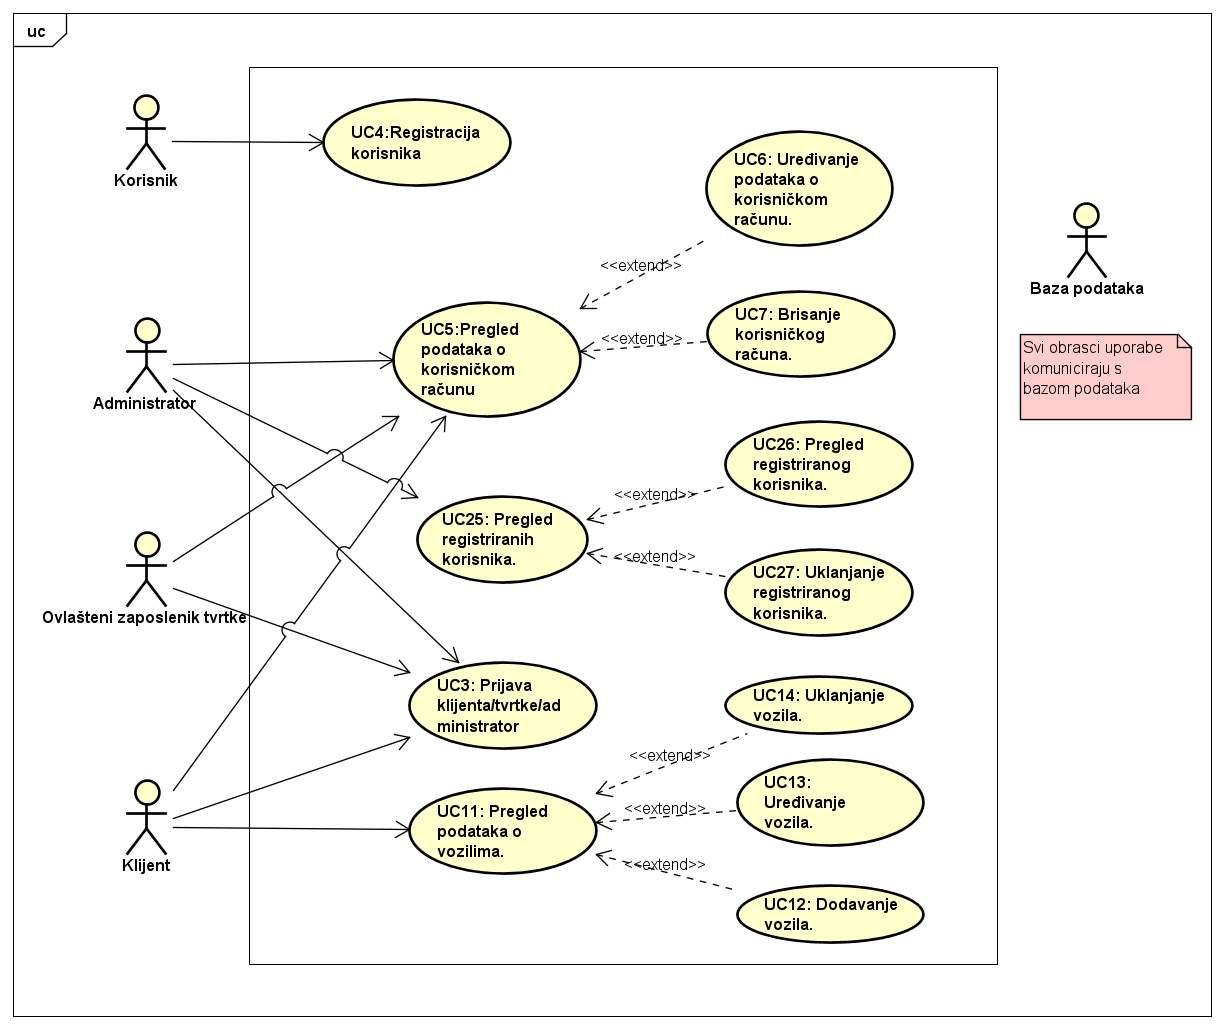
\includegraphics[width=1\linewidth]{dijagrami/Korisnički podaci.PNG} %veličina u odnosu na širinu linije
	\caption{Prikaz funkcionalnosti vezanih za korisničke podatke}
	\label{fig:promjene2} %label mora biti drugaciji za svaku sliku
\end{figure}
\begin{figure}[H]
	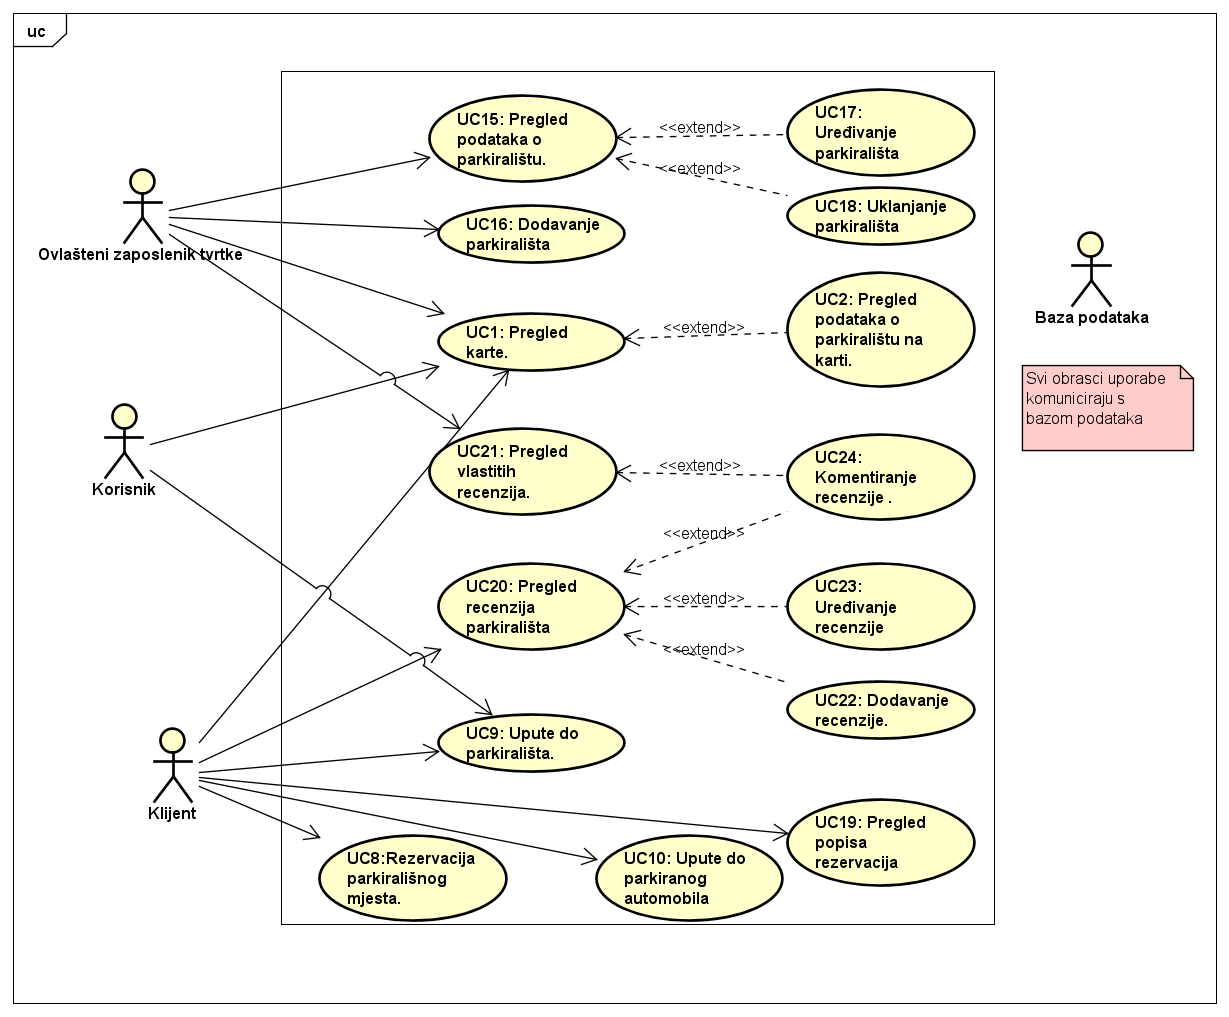
\includegraphics[width=1\linewidth]{dijagrami/Pregled ostalih funkcionalnosti.PNG} %veličina u odnosu na širinu linije
	\caption{Pregled ostalih funkcionalnosti}
	\label{fig:promjene2} %label mora biti drugaciji za svaku sliku
\end{figure}
\eject		

\subsection{Sekvencijski dijagrami}

\textbf{Obrazac uporabe UC4 - Registracija korisnika}\newline
Korisnik šalje zahtjev za registraciju. Poslužitelj prikazuje formu za popunjavanje korisničkih podataka. Korisnik unosi tražene podatke. U slučaju da neki od traženih podataka nisu validni (podaci nisu uneseni ili su uneseni neispravno) poslužitelj prikazuje odgovarajuću poruku za pojedini podatak korisnika. Ako su podaci validni, a nisu važeći (već postoji korisnik s istom e-mail adresom ili OIB-om ili brojem kartice) poslužitelj prikazuje korisniku poruku o neuspjeloj registraciji. Ako su podaci važeći poslužitelj prikazuje poruku o uspješnoj registraciji te ga automatski prijavljuje u aplikaciju.\newline
\begin{figure}[H]
	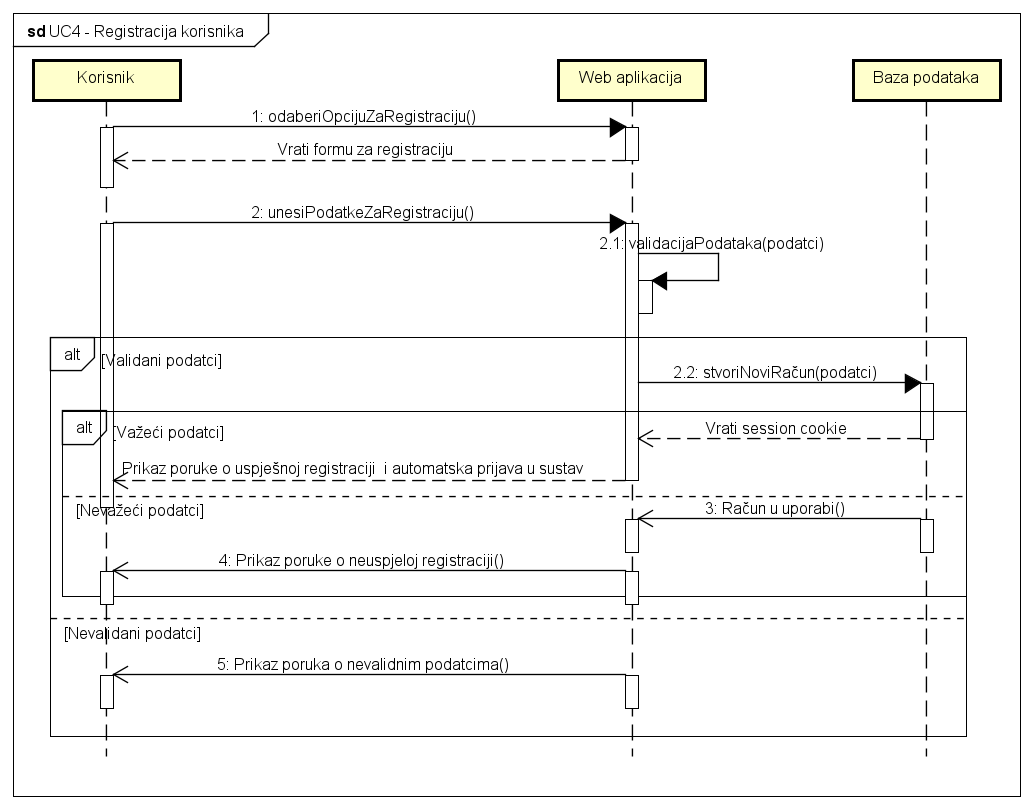
\includegraphics[width=1\linewidth]{dijagrami/UC4 - Registracija korisnika.png} %veličina u odnosu na širinu linije
	\caption{Sekvencijski dijagram za UC4}
	\label{fig:promjene2} %label mora biti drugaciji za svaku sliku
\end{figure}
\pagebreak
\textbf{Obrazac uporabe UC8 - Rezervacija parkirališnog mjesta}\newline
Klijent šalje zahtjev za prikaz karte s parkiralištima. Poslužitelj dohvaća i prikazuje prijavljena parkirališta. Odabirom parkirališta, poslužitelj iz baze podataka dohvaća osnovne podatke o parkiralištu i prikazuje ih korisniku. Kako bi obavio rezervaciju parkirališnog mjesta, klijent šalje zahtjev s tipom rezervacije i potrebne informacije vezane za rezervaciju. Poslužitelj provjerava ispravnost primljenih podatka o odabranoj rezervaciji te iz baze podataka dohvaća i provjera postoji li slobodno mjesto za traženi period na parkiralištu. Ukoliko nema slobodnih parkirališnih mjesta, sustav obavještava o tome klijenta. Ako postoji slobodno mjesto, proces rezervacije se nastavlja te se klijentu prikazuje sažetak rezervacije. Klijent tada potvrđuje plaćanje, ako kartica nema dovoljno sredstva na računu poslužitelj obavještava klijenta o neuspjelom plaćanju i vraća ga na prikaz karte. U slučaju da kartica ima dovoljno sredstva, sredstva se skidaju izravnim terećenjem. Rezervacija je završena i poslužitelj informaciju o rezervaciji prosljeđuje bazi koja sprema promjenu.\newline
\begin{figure}[H]
	\includegraphics[width=1\linewidth]{dijagrami/UC8-Rezervacija parkirališnog mjesta.png} %veličina u odnosu na širinu linije
	\caption{Sekvencijski dijagram za UC8}
	\label{fig:promjene2} %label mora biti drugaciji za svaku sliku
\end{figure}
\pagebreak
\textbf{Obrazac uporabe UC9 - Upute do parkirališta}\newline
Klijent šalje zahtjev za prikaz karte s parkiralištima. Poslužitelj dohvaća i prikazuje prijavljena parkirališta. Klijent odabire parkiralište do kojeg želi doći. Odabirom parkirališta, poslužitelj iz baze podataka dohvaća osnovne podatke o parkiralištu i prikazuje ih korisniku. Klijent šalje zahtjev za navigaciju do parkirališta. Poslužitelj otvara navigaciju te klijent dobiva upute kako doći do željenog parkirališta.
\begin{figure}[H]
	\includegraphics[width=1\linewidth]{dijagrami/UC9 - Upute do parkirališta.png} %veličina u odnosu na širinu linije
	\caption{Sekvencijski dijagram za UC9}
	\label{fig:promjene2} %label mora biti drugaciji za svaku sliku
\end{figure}
\eject

\section{Ostali zahtjevi}

\begin{packed_item}
	
	\item Sustav treba imati programsku potporu za web platformu s javnim sučeljem te prikazom karte s parkiralištima
	\item Sustav treba omogućavati istovremeni pristup za više korisnika 
	\item Programsko sučelje treba podržavati hrvatski jezik i dijakritičke znakove njegove abecede
	\item Sustav treba podržavati plaćanje u kunama
	\item Dohvat podataka iz baza mora se obaviti unutar nekoliko sekundi
	\item Sustav mora imati podršku za senzore koji očitavaju parkirna mjesta te komuniciraju s bazom podataka i redovito ju osvježavaju prilikom promjene stanja
    \item Sustav treba podržavati 3 vrste rezervacija:
        	\item[] \begin{packed_enum}
		
		\item Jednokratne rezervacije koje moraju biti napravljene barem 6 sati unaprijed te traju do 24 sata
		\item Ponavljajuće rezervacije koje moraju trajati barem 1 sat tjedno u razdoblju od minimalno mjesec dana
		\item Trajne rezervacije (0-24)
		
	\end{packed_enum}
    \item Sustav mora imati implementiranu podršku za oporavak u slučaju neispravnog korištenja korisničkog sučelja
    \item Sustav mora zabraniti pristup privatnim rutama. Ako korisnik nije bio prijavljen, preusmjerava se na formu za prijavu i ako nakon prijave ima ovlasti za tu rutu preusmjerava ga se na nju. Ako korisnik i dalje nema ovlasti ili nije bio prijavljen, preusmjerava ga se na početni zaslon aplikacije.
    \item Korisničko sučelje mora biti user friendly i jednostavno za korištenje
    \item Podaci koji se od korisnika prikupljaju i pohranjuju u bazu moraju biti zaštićeni i ograničenog pristupa
\end{packed_item}